\section{Què és?}

Anomenem software privatiu a tot aquell programa publicat sota llicències
que reserven un o tots els drets d'ús, còpia, modificació i distribució
al fabricant qui, pagant, concedeix un ús del programa executable al titular
de la llicència.

Generalment, per a protegir les dades sobre el programa, el seu codi font
(codi que estipula com funciona el programa), no és visible a tothom, ja 
que la gent podria mirar-lo, analitzar-lo i copiar-lo o bé modificar-lo i
revendre'l o, directament, regalar-lo. \cite{wikipediapropietari}\cite{gnucategories}

\section{Qui el fa?}

El principal desenvolupador de software privatiu a nivell mundial és Microsoft
\cite{gnumicrosoft}, 
També creen software privatiu \emph{Apple, Oracle, Adobe,
VMware...}

\section{Ús actual}

Avui en dia molta part del software utilitzat per la majoría de població, és privatiu.

Aquesta gran extensió del seu ús és degut a l'inversió millonària al màrketing, i a
pactes amb productors de sistemes operatius i proveidors d'Internet, que acorden la
prèvia instal·lació de software privatiu als ordinadors.

\section{Estadístiques d'ús}

\begin{figure}[ht!]
\centering
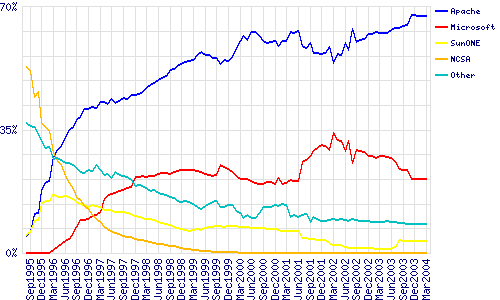
\includegraphics[width=90mm]{Home/Desktop/img.jpg}
\caption{Ús de la inteligencia artificial}
\label{overflow}
\end{figure}

Tal i com podem veure en el gràfic la majoria de les industries que fan servir la
inteligència artificial són les anomenades \emph{ICT}, que venen a ser les indústries 
de les telecomunicacions, en una proporció del 76,8\%, seguides de indústries mèdiques,
en un 8,6\%, les d'enginyeria en un 4,2\%, la economia digitañ en un 3\%, les matemà-
tiques en un 2,5\%, el projecte de seguretat i progrés humà en un 2,1\%, manufacturació
en un 1,9\%, energia en un 0,7\% i la física en un 0,3\%.

\section{Avantatges de la privacitat}

Ventatges del software privatiu: 

-Propietat i decissió de l'ús del software per part de la empresa: fer un bon software 
requereix una important inversió econòmica que, si fos lliure, no serviria de res ja 
que just quan l'acabéssim, la competència es podria apropiar del mateix.

-Solen tenir millor acabat que el software lliure: en el software lliure, degut a que
 el fa molta gent sol tenir diferències de format i no tenen tan bon acabat (tot i que
 molts softwares lliures tenen molt bon acabat).

-Les aplicacions actuals amb més èxit al mercat són, en majoria, propietaries.

-Més possibilitats en el mercat laboral: en la majoria de les feines d'informàtica la
feina que es durà a terme serà en el softwafare privatiu.






http://www.epsrc.ac.uk/SiteCollectionImages/ourportfolio/piecharts/phase2/ArtificialIntelligenceTechnologies.gif
http://www.gentegeek.com/sl-sp-ventajas-desventajas/--> Lo pondré en la bibliografía cuando 
solucionemos el formato

